\documentclass[12pt]{article}
\usepackage[english]{babel}
\usepackage{natbib}
\usepackage{url}
\usepackage[utf8x]{inputenc}
\usepackage{amsmath}
\usepackage{graphicx}
\graphicspath{{images/}}
\usepackage{parskip}
\usepackage{fancyhdr}
\usepackage{vmargin}

\usepackage{ctex}
\usepackage{multicol} %用于实现在同一页中实现不同的分栏
\usepackage{setspace} %设置行间距


%以下三个包用于给文本加边框
\usepackage{lipsum}  
\usepackage{lmodern}
\usepackage{tcolorbox}

\usepackage{multirow} %表格单元格跨行跨列
\usepackage{makecell} %使用该包的\makecell命令进行单元格内的换行


\usepackage{xcolor}


\newcommand{\tabincell}[2]{\begin{tabular}{@{}#1@{}}#2\end{tabular}}
\usepackage{listings}
\usepackage{xcolor} %要使用 listings 宏包提供的语法高亮,需要 xcolor 宏包支持

\definecolor{dkgreen}{rgb}{0,0.6,0}
\definecolor{gray}{rgb}{0.5,0.5,0.5}
\definecolor{mauve}{rgb}{0.58,0,0.82}



\lstset{ %
  language=[ANSI]C++, 					  % the language of the code
  basicstyle=\scriptsize,           % the size of the fonts that are used for the code
  numbers=left,                   % where to put the line-numbers
  numberstyle=\tiny\color{gray},  % the style that is used for the line-numbers
  stepnumber=1,                   % the step between two line-numbers. If it's 1, each line 
                                  % will be numbered
  numbersep=5pt,                  % how farCthe line-numbers are from the code
  backgroundcolor=\color{white},      % choose the background color. You must add \usepackage{color}
  showspaces=false,               % show spaces adding particular underscores
  showstringspaces=false,         % underline spaces within strings
  showtabs=false,                 % show tabs within strings adding particular underscores
  %frame=single,                   % adds a frame around the code
  frame=shadowbox,                % 为代码添加阴影边框
  rulesepcolor=\color{red!20!green!20!blue!20}, %将阴影设置为浅灰色
  %rulecolor=\color{black},        % if not set, the frame-color may be changed on line-breaks within not-black text (e.g. commens (green here))
  tabsize=2,                      % sets default tabsize to 2 spaces
  captionpos=b,                   % sets the caption-position to bottom
  breaklines=true,                % sets automatic line breaking
  breakatwhitespace=false,        % sets if automatic breaks should only happen at whitespace
  title=\lstname,                   % show the filename of files included with \lstinputlisting;
                                  % also try caption instead of title
  keywordstyle=\color{blue},          % keyword style
  commentstyle=\color{dkgreen},       % comment style
  stringstyle=\color{mauve},         % string literal style
  %escapeinside={\%*}{*)},            % if you want to add LaTeX within your code,逃逸字符
  escapeinside=``,                   %逃逸字符
  morekeywords={*,...},              % if you want to add more keywords to the set
  xleftmargin=2em,                %代码框的左边距设置为2em
  xrightmargin=2em,               %代码框的右边距设置为2em
  aboveskip=1em                   %代码框的上边距设置为1em
  %下边距采用默认值
} %插入代码框的设置,引入包+设置 

\setmarginsrb{3 cm}{2.5 cm}{3 cm}{2.5 cm}{1 cm}{1.5 cm}{1 cm}{1.5 cm}




\title{Host of Troubles Vulnerabilities}				% Title
\author{Qianyu Guo}										% Author
\date{\today}											% Date

\makeatletter
\let\thetitle\@title
\let\theauthor\@author
\let\thedate\@date
\makeatother

\pagestyle{fancy}
\fancyhf{}
\rhead{\theauthor}
\lhead{\thetitle}
\cfoot{\thepage}

\begin{document}
%%%%%%%%%%%%%%%%%%%%%%%%%%%%%%%%%%%%%%%%%%%%%%%%%%%%%%%%%%%%%%%%%%%%%%%%%%%%%%%%%%%%%%%%%

\begin{titlepage}
	\centering
    \vspace*{0.5 cm}
    
\includegraphics[scale = 0.65]{Peiyang.png}\\[1.0 cm]	% University Logo
    \textsc{\LARGE Tianjin University}\\[2.0 cm]	    % University Name
%	\textsc{\Large Course Code}\\[0.5 cm]				% Course Code
%	\textsc{\large Course Name}\\[0.5 cm]				% Course Name
	\rule{\linewidth}{0.2 mm} \\[0.4 cm]
	{ \huge \bfseries \thetitle}\\
	\rule{\linewidth}{0.2 mm} \\[1.5 cm]
	
	\begin{minipage}{0.4\textwidth}
		\begin{flushleft} \large
			\emph{Author:}\\
			\theauthor
			\end{flushleft}
			\end{minipage}~
			\begin{minipage}{0.4\textwidth}
			\begin{flushright} \large
			\emph{Student Number:} \\
			1016216001									% Your Student Number
		\end{flushright}
	\end{minipage}\\[2 cm]
	
	{\large \thedate}\\[2 cm]
 
	\vfill
	
\end{titlepage}

%%%%%%%%%%%%%%%%%%%%%%%%%%%%%%%%%%%%%%%%%%%%%%%%%%%%%%%%%%%%%%%%%%%%%%%%%%%%%%%%%%%%%%%%%

\tableofcontents
\pagebreak

%%%%%%%%%%%%%%%%%%%%%%%%%%%%%%%%%%%%%%%%%%%%%%%%%%%%%%%%%%%%%%%%%%%%%%%%%%%%%%%%%%%%%%%%%

%\section{About this design}
%This is a simple report template with the UCT logo. Feel free to use/modify it to suit your needs. Variables that need to be altered have been commented to make modifications easier. For example if you need to change the university logo, look for the comment \texttt{\% University Logo} in this file and then make appropriate modifications in that line.
%
%A Table of Contents and a bibliography have also been implemented. To add entries to your bibliography, simply edit \texttt{biblist.bib} in the root folder and then use the \texttt{\textbackslash cite\{\ldots\}} command in \texttt{main.tex} \cite{bibtex}. The Table of Contents will be updated automatically.
%
%I hope that you find this template both visually appealing and useful. \\
%
%\hspace{1 cm}--- Linus

\section{Overview}
\textbf{Host-of-Troubles} is a class of new vulnerabilities that affect a wide range of HTTP implementations. The problem is that deployed systems are generally incorrect (non-compliant with RFC 7230) and inconsistent in parsing and interpreting “Host” headers in HTTP requests. This problem can be exploited by carefully crafting HTTP requests with ambiguous host information, inducing inconsistent interpretations between two parties. Such inconsistency can lead to severe security consequences, such as HTTP cache poisoning and security policy bypass.
 \section{Multiple Host Ambiguities}
In parsing and interpreting the HTTP semantics,  one of the most important designations is what host is involved with the request, because \texttt{Host} is the key protocol field for resource locating, request routing, caching, etc. The problem of multiple host ambiguities arises when two parties (the downstream and upstream) in an HTTP processing-chain parse and interpret host in a crafted, adversarial request  differently. Inconsistency of host between two parties often causes disastrous consequences because of its semantic importance. 

\hspace{1 cm}--- \textit{Host of Troubles: Multiple Host Ambiguities in HTTP Implementations}

\subsection{Multiple Host Headers}
\label{sec:Multiple_Host_Headers}
RFC 2616\cite{rfc2616} states that a request with multiple same name headers is allowed only if the value of this header is defined as a single comma-separated list, which implies that a request with multiple \texttt{Host} headers is invalid.
RFC 7230 \cite{rfc7230} explicitly specifies that requests with multiple
\texttt{Host} headers must be reject with 400 Bad Request.

\hspace{1 cm}--- \textit{Host of Troubles: Multiple Host Ambiguities in HTTP Implementations}

\textbf{RFC 2616}
\columnseprule=1pt    %实现插入分隔线
\begin{multicols}{2}  %将该部分分两栏并在两栏列缝间插入分隔线
	\begin{spacing}{0.8} %将Specification中的部分设置为0.8倍行间距
		\textbf{4.2}
		{\footnotesize Multiple message-header fields with the same field-name MAY be present in a message if and only if the entire field-value for that header field is defined as a \textbf{comma-separated list}. It must be possible to combine the multiple header fields into one ``\texttt{field-name:field-value}" pair, without changing the semantics of the message, by appending each subsequent field-value to the first, each separated by a comma. The order in which header fields with the same field-name are received is therefore significant to the interpretation of the combined field value, and thus a proxy MUST NOT change the order of these field values when a message is forwarded. }
	
	\textbf{5.2} 
	{\footnotesize The exact resource identified by an Internet request is determined by \textbf{examining both the Request-\texttt{URI} and the \texttt{Host} header field}.\vspace{1ex}	
	%	An origin server that does not allow resources to differ by the requested host MAY ignore the Host header field value when determining the resource identified by an HTTP/1.1 request.
	An origin server that does differentiate resources based on the host requested (sometimes referred to as virtual hosts or vanity host names) MUST use the following rules for determining the requested resource on an HTTP/1.1 request:	
		\begin{enumerate}
			\item If Request-\texttt{URI} is an absolute\texttt{URI}, the host is part of the Request-\texttt{URI}. Any \texttt{Host} header field value in the request MUST be ignored.
			\item If the Request-\texttt{URI} is not an absolute\texttt{URI}, and the request includes a \texttt{Host} header field, the host is determined by the \texttt{Host} header field value.
			\item If the host as determined by rule 1 or 2 is not a valid host on the server, the response MUST be a 400 (Bad Request) error message.
		\end{enumerate}	
	Recipients of an HTTP/1.0 request that lacks a \texttt{Host} header field MAY attempt to use heuristics (e.g., examination of the URI path for something unique to a particular host) in order to determine what exact resource is being requested.}\vspace{1.2ex}
	\textbf{14.23}
	{\footnotesize A client MUST include a \texttt{Host} header field in all HTTP/1.1 request messages . If the requested \texttt{URI} does not include an Internet host name for the service being requested, then the \texttt{Host} header field MUST be given with an empty value. An HTTP/1.1 proxy MUST ensure that any request message it forwards does contain an appropriate \texttt{Host} header field that identifies the service being requested by the proxy. All Internet-based HTTP/1.1 servers MUST respond with a 400 (Bad Request) status code to any HTTP/1.1 request message which lacks a \texttt{Host} header field.}
	
	\textbf{19.6.1.1}
	{\footnotesize It is extremely important that all implementations of HTTP (including updates to existing HTTP/1.0 applications) correctly implement these requirements:
		\begin{itemize}
			\item Both clients and servers MUST support the \texttt{Host} request-header.
			\item A client that sends an HTTP/1.1 request MUST send a \texttt{Host} header.
			\item Servers MUST report a 400 (Bad Request) error if an HTTP/1.1
				request does not include a \texttt{Host} request-header.
			\item Servers MUST accept absolute \texttt{URIs}.
		\end{itemize}
		}
	\end{spacing}
\end{multicols}

\textbf{RFC 7230}
\columnseprule=1pt    %实现插入分隔线
\begin{multicols}{2}
	\begin{spacing}{0.8}
	\textbf{3.2.2}
	{\footnotesize A sender MUST NOT generate multiple header fields with the same field name in a message unless either the entire field value for that header field is defined as a comma-separated list [i.e., \#(values)] or the header field is a well-known exception.}
	
	\textbf{5.4}
	{\footnotesize A server MUST respond with a 400 (Bad Request) status code to any HTTP/1.1 request message that \textbf{lacks a Host header} field and to any request message that \textbf{contains more than one Host header} field or a Host header field with an \textbf{invalid field-value}.}
	\end{spacing}
\end{multicols}

\subsection{Space-surrounded Host Header}
\subsubsection{The first header with preceding space}
RFC 2616 does not have explicit text for this case. The syntax definition implies that systems should reject the request with a space preceding the first header. RFC 7230 suggests to either reject the request or ignore the header.

\textbf{RFC 2616}
\columnseprule=1pt    %实现插入分隔线
\begin{multicols}{2}
	\begin{spacing}{0.8}
		\textbf{} 
		{\footnotesize  }
	\end{spacing}
\end{multicols}

\textbf{RFC 7230}
\columnseprule=1pt    %实现插入分隔线
\begin{multicols}{2}
	\begin{spacing}{0.8}
		\textbf{3.} 
		%关于前带空格的header的处理
		{\footnotesize 
		A sender MUST NOT send whitespace between the start-line and the
		first header field. \textbf{A recipient that receives whitespace between the start-line and the first header field MUST either reject the message} as invalid or consume each whitespace-preceded line without further processing of it (i.e., \textbf{ignore the entire line}, along with any subsequent lines preceded by whitespace, until a properly formed header field is received or the header section is terminated).\vspace{1ex} \\ 
		The presence of such whitespace in a request might be an attempt to trick a server into ignoring that field or processing the line after it as a new request, either of which might result in a security vulnerability if other implementations within the request chain interpret the same message differently.\\	
		}
		\textbf{3.2.4} 
	    {\footnotesize  The field value does not include any leading or trailing whitespace: \textbf{OWS occurring before the first non-whitespace octet of the field value} or after the last non-whitespace octet of the field value \textbf{ought to be excluded} by parsers when extracting the field value from a header field.}
	\end{spacing}
\end{multicols}

\subsubsection{Non-first header with preceding space}
RFC 2616 states that a such header needs to be processed as folded line of its previous header: remove its preceding line break characters to concatenate with the
previous header. Although RFC 7230 already obsoletes line folding, it still allows a proxy or a server to process as line folding for backward compatibility considerations.

\hspace{1 cm}--- \textit{Host of Troubles: Multiple Host Ambiguities in HTTP Implementations}

\textbf{RFC 2616}
\columnseprule=1pt    %实现插入分隔线
\begin{multicols}{2}
	\begin{spacing}{0.8}
		\textbf{2.2} 
		{\footnotesize  \textbf{HTTP/1.1 header field values can be folded onto multiple lines if the continuation line begins with a space or horizontal tab.} All linear white space, including folding, has the same semantics as SP. A recipient MAY replace any linear white space with a single SP before interpreting the field value or forwarding the message downstream. }
	\end{spacing}
\end{multicols}

\textbf{RFC 7230}
\columnseprule=1pt    %实现插入分隔线
\begin{multicols}{2}
	\begin{spacing}{0.8}
		\textbf{3.2.4} 
		{\footnotesize Historically, HTTP header field values could be extended over
		multiple lines by preceding each extra line with at least one space or horizontal tab (obs-fold).\textbf{ This specification deprecates such line folding except within the message/http media type.}}
	\end{spacing}
\end{multicols}

\subsubsection{Headers with succeeding space}
RFC 2616 does not have explicit text for this case. The syntax definition implies that systems should allow this request. The same situation is explicitly forbidden in RFC 7230.

\textbf{RFC 2616}
\columnseprule=1pt    %实现插入分隔线
\begin{multicols}{2}
	\begin{spacing}{0.8}
		\textbf{} 
		{\footnotesize  }
	\end{spacing}
\end{multicols}

\textbf{RFC 7230}
\columnseprule=1pt    %实现插入分隔线
\begin{multicols}{2}
	\begin{spacing}{0.8}
		\textbf{3.2.4} 
		{\footnotesize  A field value might be preceded and/or followed by optional
			whitespace (OWS). The field value does not include any leading or trailin whitespace: \textbf{OWS occurring} before the first non-whitespace octet of the field value or \textbf{after the last non-whitespace octet of the field value ought to be excluded} by parsers when extracting the field value from a header field.}
	\end{spacing}
\end{multicols}

\begin{figure*}[!htbp]
	\centering
	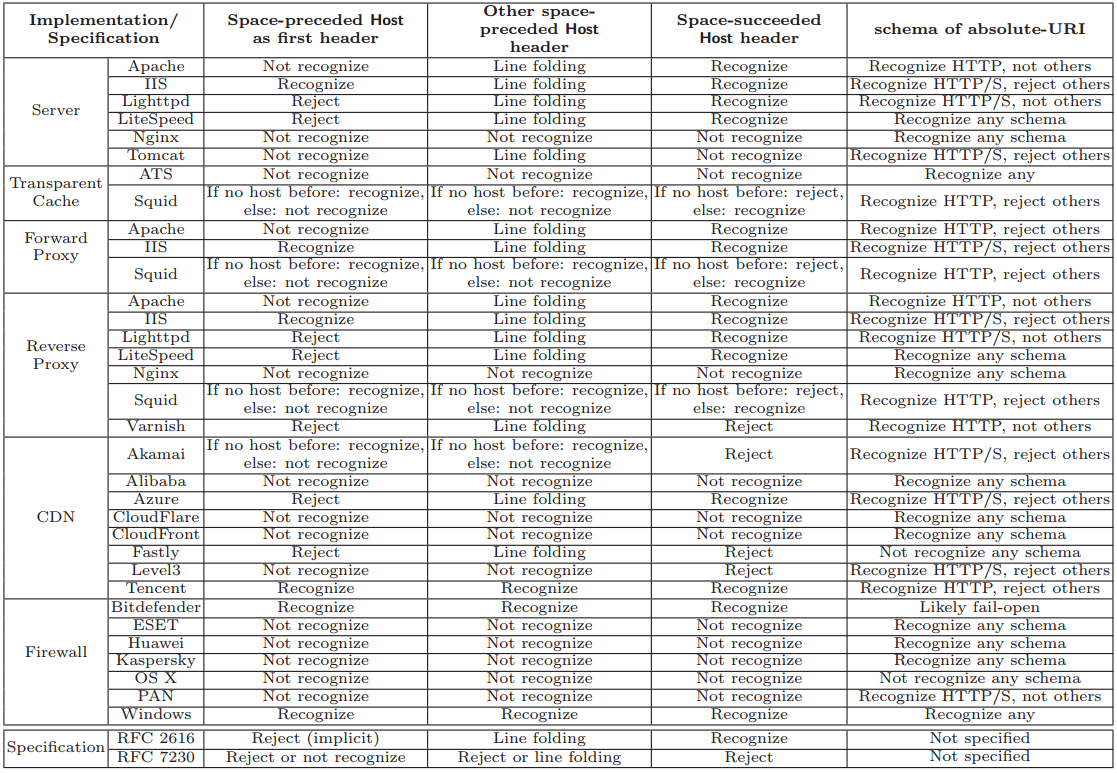
\includegraphics[width=1.0\textwidth]{Host_Parsing.jpg}
	\caption{Host parsing behaviors. Specifications and tested implementations (``recognize" means accepting as valid host field, ``not recognize" means either ignoring or accepting as an unknown header field, ``reject" means responding with 400 Bad Request).}
	\label{fig:host_parsing}
\end{figure*}
\subsection{Absolute-URI as Request-Target}
Both RFC 2616 and RFC 7230 require server to accept absolute-\texttt{URI} as request-target, and to prefer host component of absolute-\texttt{URI} than \texttt{Host} header. RFC 7230 additionally requires requests with absolute-URI to have identical host component as \texttt{Host} header. Both of the two RFCs do not explicitly state which schema is allowed in the absolute-URI.

\textbf{RFC 2616}
\columnseprule=1pt    %实现插入分隔线
\begin{multicols}{2}
	\begin{spacing}{0.8}
		\textbf{5.2} 
		{\footnotesize See the ``RFC 2616" part in section \ref{sec:Multiple_Host_Headers}.}
	\end{spacing}
\end{multicols}

\textbf{RFC 7230}
\columnseprule=1pt    %实现插入分隔线
\begin{multicols}{2}
	\begin{spacing}{0.8}
		\textbf{5.5} 
		{\footnotesize 
		\textbf{Since the request-target often contains only part of the user agent’s target URI, a server reconstructs the intended target as an ``effective request URI" to properly service the request}. This reconstruction involves both the \textbf{server’s local configuration} and information communicated in the \textbf{request-target}, \textbf{\texttt{Host} header field}, and \textbf{connection context}.\vspace{1.2ex}\\
		For a user agent, the effective request URI is the target URI. If the request-target is in absolute-form, the effective request URI is the same as the request-target. Otherwise, the effective request URI is constructed as follows:
	
		\begin{enumerate}
			\item If the server’s configuration (or outbound gateway) provides a
			fixed URI \textbf{scheme}, that scheme is used for the effective request URI. Otherwise, if the request is received over a TLS-secured TCP connection, the effective request URI’s scheme is "https"; if not, the scheme is "http".
			\item If the server’s configuration (or outbound gateway) provides a fixed URI \textbf{authority component}, that authority is used for the effective request URI. If not, then if the request-target is in authority-form, the effective request URI’s authority component is the same as request-target. If not, then if a \texttt{Host} header field is supplied with a non-empty field-value, the authority component is the same as the \texttt{Host} field-value. Otherwise, the authority component is assigned the default name configured for the server and, if the connection’s incoming TCP port number differs from the default port for the effective request URI’s scheme, then a colon (":") and the incoming port number are appended to the authority component.
			\item If the request-target is in authority-form or asterisk-form, the
			effective request URI’s combined path and query component is empty. Otherwise, the combined path and query component is the same as the request-target.
		
		\end{enumerate}
	
		The components of the effective request URI, once determined as above, can be combined into absolute-URI form by concatenating the \textbf{scheme}, "://", \textbf{authority}, and \textbf{combined path and query component}. }
	\end{spacing}
\end{multicols}	
	


\newpage
\section{Case Studies}
\subsection{Multiple Host Headers}

\textbf{Case 1} 讨论当同一个Request中存在多个Host字段时,该如何解析和处理。
\vspace{1ex}

\begin{spacing}{0.8}
	\begin{tcolorbox}
	
		\textbf{RFC 2616}
		Multiple message-header fields with the same \texttt{field-name} {\color{red}{MAY}} be present in a message {\color{red}{ if and only if (隐晦地说明Multiple Host是不允许的)}} the entire \texttt{field-value} for that header field is defined as a comma-separated list. It MUST be possible to combine the multiple header fields into one ``\texttt{field-name: field-value}'' pair, without changing the semantics of the message, by appending each subsequent field-value to the first, each separated by a comma. (Page 22, 4.2, Meassage Headers)
	\end{tcolorbox}
\end{spacing} 

\vspace{1ex}

\begin{spacing}{0.8}
		\begin{tcolorbox}
		\textbf{RFC 7230} 
		A sender {\color{red}{MUST NOT}} generate multiple header fields with the same field name in a message unless either the entire field is defined  as a comma-separated list ...
	
		A recipient MAY combine multiple header fields with the same field name into one ``\texttt{field-name: field-value}'' pair, without changing the semantics of the message, by appending each subsequent field value to the combined field value in order, separated by a comma. (Page 24, 3.2.2, Field Order)
	\end{tcolorbox}
\end{spacing}

\vspace{1ex}

\begin{spacing}{0.8}
	\begin{tcolorbox}
		\textbf{RFC 7230}
		A server {\color{red}{MUST respond with a 400 (Bad Request)}} status code to any HTTP/1.1 request message that lacks a \texttt{Host} header field and to any request message that {\color{red}{contains more than one \texttt{Host} header field}} or a \texttt{Host} header field with an invalid field-value. (Page 44, 5.4,  Host)
	\end{tcolorbox}
\end{spacing}

\vspace{2ex}

\begin{figure*}[!htbp]
	\centering
	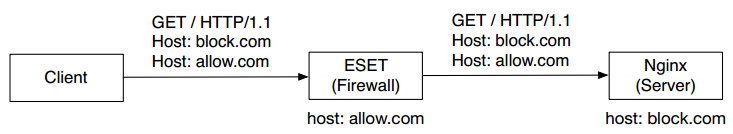
\includegraphics[width=1.0\textwidth]{Preference_Multi-Host.jpg}
	\caption{Preference of multiple \texttt{Host} headers.}
	\label{fig:preference_multi-Host}
\end{figure*}

首先,在同一个Request中出现多个\texttt{Host}本来就是非法的,而ESET和Nginx都允许这种情况出现。其次,面对多个\texttt{Host},二者选择的方式不一样,见下表:

\begin{table}[!htbp]
	\renewcommand\arraystretch{1} 
	\begin{tabular}{|c|c|c|}
		\hline 
		\textbf{Implementation} & \makecell{\textbf{Preference} \\ \textbf{for multiple \texttt{Host}}} & \makecell{\textbf{Request forwarding} \& \\ \textbf{Host interpreting}}  \\  
		\hline 
		ESET & \textbf{Last} \texttt{Host} & 原样转发 \\ 
		\hline 
		Nginx & \textbf{First} \texttt{Host} & \\
		\hline
		\hline
		RFC 2616 & Reject & \\
		\hline
		RFC 7230 & Reject & \makecell{ Absolute-URI中的Host优先\\为Absolute-URI新建一个Host字段\\ Host字段其次} \\
		\hline
	\end{tabular} 
\caption{Case 1}
\end{table}

\textbf{Case 2} 讨论如果Request中同时存在Absolute-URI和Host字段,该如何解析和处理。
\begin{spacing}{0.8}
	\begin{tcolorbox}
		\textbf{RFC 2616}
		An origin server that does differentiate resources based on the host requested MUST use the following rules for determining the requested resource on an HTTP/1.1 request:
		\begin{enumerate}
			\item If \texttt{Request-URI} is an \texttt{absoluteURI}, the host is part of the \texttt{Request-URI}. Any \texttt{Host} header field value in the request MUST be ignored.
			\item If the \texttt{Request-URI} is not an \texttt{absoluteURI}, and the request includes a \texttt{Host} header field, the host is determined by the \texttt{Host} header field value.
			\item If the host as determined by rule 1 or 2 is not a valid host on the server, the response MUST be a 400 (Bad Request) error message. (Page 25, 5.2, The Resource Identified by a Request)
		\end{enumerate}
	\end{tcolorbox}
\end{spacing}
\vspace{1ex}
\begin{spacing}{0.8}
	\begin{tcolorbox}
		\textbf{RFC 7230 有关如何解析Host和转发Request}
		
		When a proxy receives a request with an absolute-form of request-target, the proxy MUST ignore the received \texttt{Host} header field (if any) and instead replace it with the host information of the
		request-target (Absolute-URI中的Host信息优先). A proxy that forwards such a request {\color{red}{MUST generate a new Host field-value based on the received request-target}} rather than forward the received \texttt{Host} field-value. (Page 44, 5.4, Host)
	\end{tcolorbox}
\end{spacing}

总结起来就是说:如果有\texttt{Absolute-URI},则取这里面的Host,\texttt{Host}字段中的值被忽略。如果没有\texttt{Absolute-URI},则以\texttt{Host}字段的值为准。否则,报错400 Bad Request。

\begin{figure*}[!htbp]
	\centering
	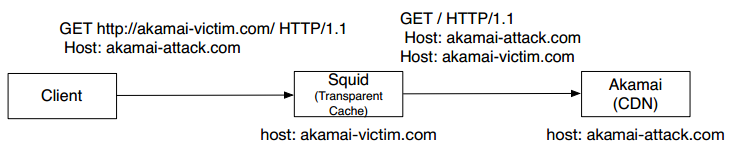
\includegraphics[width=1.0\linewidth]{images/AbsoluteURI_Host}
	\caption{Absolute URI with \texttt{Host} headers.}
	\label{fig:absolute-uri_host}
\end{figure*}

\begin{table}[!htbp]
	\renewcommand\arraystretch{1}
	\centering
	\begin{tabular}{|l|c|c|c|l|c|}
		\hline
		\multicolumn{2}{|c}{\multirow{3}{*}{\tabincell{l}{Implementation\\/Specification}}} & 
		\multicolumn{2}{|c|}{\multirow{2}{*}{\tabincell{l}{Prefer Absolute-URI\\vs. Prefer Host header}}} &
		\multicolumn{1}{c|}{\multirow{3}{*}{Request forwarding}} &
		\multicolumn{1}{c|}{\multirow{3}{*}{\tabincell{c}{Preference\\for multiple\\Host}}}
		\\ 
		\multicolumn{2}{|l|}{} & \multicolumn{2}{c|}{} & &
		\\ \cline{3-4}
		\multicolumn{2}{|l|}{} & \textbf{Preference} & \textbf{Consistency} & &
		\\ \hline
		Squid & \tabincell{c}{Transparent\\Cache} & Absolute-URI & Optional & {\tabincell{l}{1.Generate a new \\ Host header \\for Absolute-URI \\and select this one. \\ 2.Forward\\ space-preceded \\Host headers as-is}} & Prefer first
		\\ \hline
		Akamai & CDN & Host header & Optional & & Prefer first
		\\ \hline
		\hline
		\multicolumn{1}{|c|}{\multirow{2}{*}{Specification}}  & RFC 2616 & Absolute-URI & Not Specified & & Reject
		\\ \cline{2-6}
		& RFC 7230 & Absolute-URI & Must & & Reject
		\\ \hline
	\end{tabular}
\caption{Case 2}
\end{table}

\pagebreak
\textbf{Case 3} 讨论多Host header,同时伴随前置空格(preceding space)的情况。
\begin{spacing}{0.8}
	\begin{tcolorbox}
		\textbf{RFC 7230}
		A field value {\color{red}{might}} be preceded and/or followed by optional whitespace (OWS); a single SP preceding the field-value is preferred for consistent readability by humans. The field value does not include any leading or trailing whitespace: OWS occurring before the first non-whitespace octet of the field value or after the last non-whitespace octet of the field value ought to be excluded by parsers when extracting the field value from a header field. (Page 25, 3.2.4, Field Parsing) {\color{red}{隐约地说明field value最前头或最后头有空格是允许的!}}
	\end{tcolorbox}
\end{spacing}

\begin{figure}[!htbp]
	\centering
	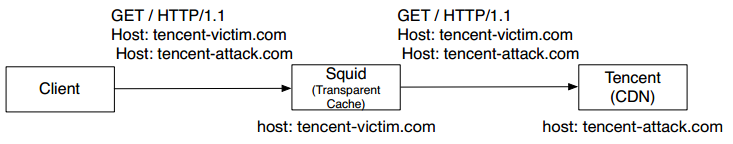
\includegraphics[width=1.0\linewidth]{images/Multi-Host_Preceding_Space}
	\caption{Multiple \texttt{Host} headers with preceding space.}
	\label{fig:multi-host_precedingspace}
\end{figure}
 
\begin{table}[!htbp]
	\renewcommand\arraystretch{1}
	\begin{tabular}{|c|c|c|c|c|}
		\hline
		\multicolumn{2}{|c|}{\multirow{2}{*}{\tabincell{l}{Implementation\\/Specification}}} & 
	\multirow{2}{*}{\tabincell{c}{Space-preceded Host\\ as first Host header}} &
	\multirow{2}{*}{\tabincell{c}{Other Space-preceded\\Host header}} &
	\multirow{2}{*}{\tabincell{c}{Space-succeeded\\Host header}} 
	\\ 
	\multicolumn{2}{|c|}{} & \multirow{2}{*}{} & \multirow{2}{*}{}& \multirow{2}{*}{}
	\\ \hline
	Squid & \tabincell{c}{Transparent\\Cache} & \tabincell{l}{If no Host header \\ before:recognize \\ Else: {\color{red}{not recognize}}} & \tabincell{l}{If no Host header\\before:recognize\\Else: not recognize} & \tabincell{l}{If no Host header\\before:recognize\\Else: not recognize}
	\\ \hline
	Tencent & CDN & Recognize & Recognize & Recognize 
	\\ \hline \hline 
	\multirow{2}{*}{Specification}  & RFC 2616 & Reject & Line folding & Recognize 
	\\ \cline{2-5}
	& RFC 7230 & Recognize & Recognize & Recognize 
	\\ \hline
\end{tabular}
\caption{Case 3-1, {\color{red}{Recognize: accepting as valid host field}},{\color{red}{Reject: 400 Bad Requests}}, {\color{red}{Reject: Not recognize:either ignoring or accepting as an unknown header field}}.}
\end{table}

\begin{table}[!htbp]
	\renewcommand\arraystretch{1}
	\centering
	\begin{tabular}{|c|c|c|}
		\hline
		\multicolumn{2}{|c|}{\multirow{2}{*}{Implementation/Specification}} &
		\multirow{2}{*}{Preference for multiple Host}
		\\ 
		\multicolumn{2}{|c|}{} & 
		\\ \hline
		Squid & Transparent Cache & Prefer first 
		\\ \hline
		Tencent & CDN & Prefer last
		\\ \hline \hline
		\multirow{2}{*}{Specification} & RFC 2616 & Reject
		\\ \cline{2-3}
		& RFC 7230 & Reject
		\\ \hline
	\end{tabular}
\caption{Case 3-2}
\end{table}


Case 4: 讨论RFC Ambiguities可能出现的地方
\begin{spacing}{0.8}
	\begin{tcolorbox}
		\textbf{RFC 7230} A field value might be preceded and/or followed by optional whitespace (OWS) ...
	\end{tcolorbox}
\end{spacing}

\vspace{1ex}

\begin{spacing}{0.8}
	\begin{tcolorbox}
		A server that receives an obs-fold in a request message MUST {\color{red}{either}} reject the message by
		sending a 400 (Bad Request) ... {\color{red}{or}} replace each received obs-fold with one or more SP octets prior to interpreting the field value {\color{red}{or}} forwarding the message downstream.
		
		A proxy or gateway MUST {\color{red}{either}} discard the message and replace it with a 502 (Bad Gateway) response {\color{red}{or}} replace each received obs-fold with one {\color{red}{or}} more SP octets prior to interpreting the field value or forwarding the message downstream.  (Page 25-26, 3.2.4, Field Parsing)
	\end{tcolorbox}
\end{spacing}

\vspace{1ex}

\begin{spacing}{0.8}
	\begin{tcolorbox}
	A proxy or gateway MUST {\color{red}{either}} discard the message and replace it with a 502 (Bad Gateway) response {\color{red}{or}} replace each received obs-fold with one {\color{red}{or}} more SP octets prior to interpreting the field value or forwarding the message downstream.  (Page 26, 3.2.4, Field Parsing)
	\end{tcolorbox}
\end{spacing}
\newpage
\section{Implementation}

\begin{table}[htbp!]
	\centering
	\renewcommand\arraystretch{1}
	\begin{tabular}{|c|c|c|c|}
		\hline 
		\textbf{ Intermediates} & \textbf{Source Code Website} & \textbf{Version} & \textbf{Category} \\ 
		\hline 
		\hline 
		Squid & http://www.squid-cache.org & 3.5.12 & \makecell{Transparent Cahce\\Forward Proxy\\Reverse Proxy} \\ 
		\hline 
		Apache & https://httpd.apache.org & &\makecell{Server\\ Forward Proxy\\ Reverse Proxy}\\
		\hline
	\end{tabular} 
\end{table}


\begin{lstlisting}[title= squid/src/HttpRequest.cc line:339]
int HttpRequest::parseHeader(const char *parse_start, int len)
{
  const char *blk_start, *blk_end;
  if (!httpMsgIsolateHeaders(&parse_start, len, &blk_start, &blk_end))
  return 0;

  int result = header.parse(blk_start, blk_end);

  if (result)
  hdrCacheInit();
  return result;
}
\end{lstlisting}

\begin{lstlisting}[title=squid/src/HttpHeader.cc line:588]
int HttpHeader::parse(const char *header_start, const char *header_end)
{
  ...
  if ((e = HttpHeaderEntry::parse(field_start, field_end)) == NULL) //line 684
  ...
}
\end{lstlisting}

\begin{lstlisting}[title= squid/src/HttpHeader.cc line:1620]
/* parses and inits header entry, returns true/false */
HttpHeaderEntry * HttpHeaderEntry::
parse(const char *field_start, const char *field_end)
{
  /* note: name_start == field_start */
  const char *name_end = (const char *)memchr(field_start, ':', field_end - field_start);
  int name_len = name_end ? name_end - field_start :0;
  const char *value_start = field_start + name_len + 1; // skip ':' 
  /* note: value_end == field_end */
  ...
  /* now we know we can parse it */
  ...
  /* is it a "known" field? */
  // Header ID
  http_hdr_type id = httpHeaderIdByName(field_start, name_len, Headers, HDR_ENUM_END);
  String name;  // Header name
  String value; // Header value
  if (id < 0)
  id = HDR_OTHER;
  assert_eid(id);
  
  /* set field name */
  if (id == HDR_OTHER)
  name.limitInit(field_start, name_len);
  else
  name = Headers[id].name;
  
  /* trim field value */
  while (value_start < field_end && xisspace(*value_start))
  ++value_start;
  
  while (value_start < field_end && xisspace(field_end[-1]))
  --field_end;
  ...

  /* set field value */
  value.limitInit(value_start, field_end - value_start);
  
  debugs(55, 9, "parsed HttpHeaderEntry: '" << name << ": " << value << "'");
  
  return new HttpHeaderEntry(id, name.termedBuf(), value.termedBuf());
}
\end{lstlisting}

\begin{lstlisting}[title=squid/src/client\_side.cc line:2152]
ClientSocketContext *
parseHttpRequest(ConnStateData *csd, HttpParser *hp, HttpRequestMethod * method_p, Http::ProtocolVersion *http_ver)
{
	...
	/* Attempt to parse the first line; this'll define the method, url, version and header begin */
	r = HttpParserParseReqLine(hp);
	...
	/* Rewrite the URL in transparent or accelerator mode */
	/* NP: there are several cases to traverse here:
	*  - standard mode (forward proxy)
	*  - transparent mode (TPROXY)
	*  - transparent mode with failures
	*  - intercept mode (NAT)
	*  - intercept mode with failures
	*  - accelerator mode (reverse proxy)
	*  - internal URL
	*  - mixed combos of the above with internal URL
	*  - remote interception with PROXY protocol
	*  - remote reverse-proxy with PROXY protocol
	*/
	if (csd->transparent()) {
		/* intercept or transparent mode, properly working with no failures */
		prepareTransparentURL(csd, http, url, req_hdr);
	} else if (internalCheck(url)) {
		/* internal URL mode */
		/* prepend our name & port */
		http->uri = xstrdup(internalLocalUri(NULL, url));
		// We just re-wrote the URL. Must replace the Host: header.
		//  But have not parsed there yet!! flag for local-only handling.
		http->flags.internal = true;
	
		} else if (csd->port->flags.accelSurrogate || csd->switchedToHttps()) {
		/* accelerator mode */
		prepareAcceleratedURL(csd, http, url, req_hdr);
	}
}
\end{lstlisting}




\begin{lstlisting}[title=squid/src/client\_side.cc  line:2110 prepareTransparentURL()] 
static void
prepareTransparentURL(ConnStateData * conn, ClientHttpRequest *http, char *url, const char *req_hdr)
{
	char *host;
	char ipbuf[MAX_IPSTRLEN];
	
	if (*url != '/')
	return; /* already in good shape */
	
	/* BUG: Squid cannot deal with '*' URLs (RFC2616 5.1.2) */
	
	if ((host = mime_get_header(req_hdr, "Host")) != NULL) 
	{
		int url_sz = strlen(url) + 32 + Config.appendDomainLen +
		strlen(host);
		http->uri = (char *)xcalloc(url_sz, 1);
		snprintf(http->uri, url_sz, "%s://%s%s", AnyP::UriScheme(conn->port->transport.protocol).c_str(), host, url);
		debugs(33, 5, "TRANSPARENT HOST REWRITE: '" << http->uri <<"'");
	} 
	else 
	{
		/* Put the local socket IP address as the hostname.  */
		int url_sz = strlen(url) + 32 + Config.appendDomainLen;
		http->uri = (char *)xcalloc(url_sz, 1);
		http->getConn()->clientConnection->local.toHostStr(ipbuf,MAX_IPSTRLEN);
		snprintf(http->uri, url_sz, "%s://%s:%d%s",
		AnyP::UriScheme(http->getConn()->port->transport.protocol).c_str(),
		ipbuf, http->getConn()->clientConnection->local.port(), url);
		debugs(33, 5, "TRANSPARENT REWRITE: '" << http->uri << "'");
	}
}
\end{lstlisting}

\begin{lstlisting}[title=squid/src/mime\_header.cc  line:89]
/* returns a pointer to a field-value of the first matching field-name */
char * mime_get_header(const char *mime, const char *name)
{
	return mime_get_header_field(mime, name, NULL);
}
\end{lstlisting}


\begin{lstlisting}[title=squid/src/mime\_header.cc  line:22]
/*
* returns a pointer to a field-value of the first matching field-name where
* field-value matches prefix if any
*/
char * mime_get_header_field(const char *mime, const char *name, const char *prefix)
{
	LOCAL_ARRAY(char, header, GET_HDR_SZ);
	const char *p = NULL;
	char *q = NULL;
	char got = 0;
	const int namelen = name ? strlen(name) : 0;
	const int preflen = prefix ? strlen(prefix) : 0;
	int l;
	...
	for (p = mime; *p; p += strcspn(p, "\n\r")) {
		if (strcmp(p, "\r\n\r\n") == 0 || strcmp(p, "\n\n") == 0)
			return NULL;

		//Squid表现:If no host before: recognize. Else not recognize.
		while (xisspace(*p))  //Space-preceded Host Host前方有空格的解析 
			++p;

		if (strncasecmp(p, name, namelen))
			continue;
		if (!xisspace(p[namelen]) && p[namelen] != ':')
			continue;
		l = strcspn(p, "\n\r") + 1;
		if (l > GET_HDR_SZ)
			l = GET_HDR_SZ;

		xstrncpy(header, p, l);
		q = header;
		q += namelen;
		if (*q == ':') {
			++q;
			got = 1;
		}

		///Squid表现:If no host before: reject. Else not recognize. 有矛盾?
		while (xisspace(*q)) { //Space-succeeded Host Host后方有空格的解析 
			++q;
			got = 1;
		}

		if (got && prefix) {
			/* we could process list entries here if we had strcasestr(). */
			/* make sure we did not match a part of another field-value */
			got = !strncasecmp(q, prefix, preflen) && !xisalpha(q[preflen]);
		}

		if (got) {
			debugs(25, 5, "mime_get_header: returning '" << q << "'");
			return q;
		}
	}
	return NULL;
}
\end{lstlisting}


\newpage
\bibliographystyle{plain}
\bibliography{biblist}

\end{document}